\chapter{Los n\'umeros de Fibonacci: un ejemplo del \'area de \'Algebra}
\label{CapituloFibonacci}

En este cap\'\i tulo damos una f\'ormula expl\'\i cita para los n\'umeros de la sucesi\'on de Fibonacci\footnote{\emph{Leonardo de Pisa, Fibonacci}, Pisa, 1170-1250.}
 como aplicaci\'on de la teor\'\i a de diagonalizaci\'on de matrices.

\section{La sucesi\'on de Fibonacci}
\label{Seccion1}

La sucesi\'on de Fibonacci es una sucesi\'on bien conocida, incluso en \'ambitos ajenos a las matem\'aticas.

\begin{definicion} La \emph{sucesi\'on de Fibonacci} $\{F_n\}$ es la sucesi\'on de n\'umeros definida por los valores iniciales $F_1=F_2=1$ y por la relaci\'on de recurrencia
\begin{equation}\label{Fibonacci}F_n=F_{n-1}+F_{n-2},\ \ \text{para } n>2.\end{equation}
\end{definicion}

Sus primeros t\'erminos son por lo tanto:
$$1,\  1,\  2,\  3,\  5,\  8,\  13,\  21,\  34,\  55,\  89,\dots $$

Observamos que los n\'umeros de Fibonacci, al menos los primeros, crecen con cierta rapidez y no es dif\'\i cil dar una explicaci\'on a este hecho. En efecto, la sucesi\'on de Fibonacci es claramente creciente, por lo tanto, si $n>2$,
$$F_n=F_{n-1}+F_{n-2}\geq 2F_{n-2}.$$
Iterando esta desigualdad obtenemos que $F_{2k}\geq 2^{k-1}$  y $F_{2k-1}\geq 2^{k-1}$, es decir,
$F_n\geq 2^{\lceil n/2\rceil-1}$, donde $\lceil\ \rceil$ denota la funci\'on techo ($\lceil x\rceil$ es el menor entero mayor o igual que $x$).

La gr\'afica de la Figura \ref{grafica}  muestra los puntos $(n,\log F_n)$ para $n=1,\dots,25$.  El aspecto de esta gr\'afica sugiere fuertemente que los n\'umeros de Fibonacci crecen exponencialmente. En efecto, salvo para los primeros valores, los puntos parecen estar sobre una recta, digamos la de ecuaci\'on $y=ax+b$, lo cual quiere decir que $\log F_n\approx an+b$, esto es $F_n\approx A\cdot B^n$ para algunas constantes $A$ y $B$. N\'otese que, ciertamente, se trata de una aproximaci\'on pero en ning\'un caso de una igualdad. Si fuera as\'\i\ se tendr\'\i a que $F_n/F_{n-1}$ ser\'\i a constante (igual a $B$), lo que claramente es falso. En todo caso deber\'\i a tenerse que $\lim_{n\to\infty} F_n/F_{n-1}=B$. Confirmaremos este hecho al final del cap\'\i tulo.

\begin{figure}
\begin{center}
\scalebox{1}{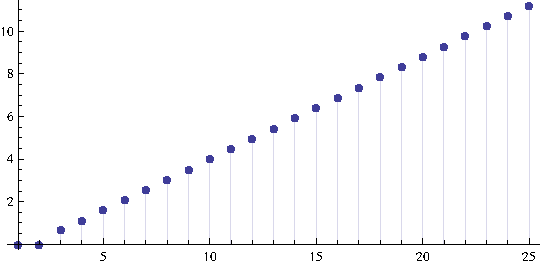
\includegraphics{grafica.pdf}}
\end{center}
\caption{\label{grafica} Los puntos $(n,\log F_n)$ para $n=1,\dots,25$.}
\end{figure}



\section{Una f\'ormula expl\'\i cita para los n\'umeros de Fibonacci}

N\'otese que si definimos $F_0=0$, la f\'ormula de recurrencia (\ref{Fibonacci}) junto con los valores iniciales $F_0=0$, $F_1=1$ determinan tambi\'en los n\'umeros de la sucesi\'on de Fibonacci $F_n$.

Consideremos ahora la matriz $A=\begin{pmatrix} 0&1\\ 1&1\end{pmatrix}=\begin{pmatrix} F_0&F_1\\ F_1&F_2\end{pmatrix}$.

Un sencillo argumento inductivo prueba que
\begin{equation}\label{FormulaPotenciaN} A^n=\begin{pmatrix} F_{n-1}&F_n\\ F_n&F_{n+1}\end{pmatrix},\ \text{para todo } n\geq 1.\end{equation}

La idea es calcular ahora $A^n$ expl\'\i citamente diagonalizando primero la matriz $A$.

\begin{teorema} Sea $A$ la matriz definida anteriormente. Entonces $A=PDP^{-1}$, donde
$$D=\begin{pmatrix} \Phi&0\\ 0&-1/\Phi\end{pmatrix}\quad \text{y}\quad P=\begin{pmatrix} 1&1\\ \Phi &-1/\Phi\end{pmatrix},$$
siendo $\displaystyle \Phi=\frac{1+\sqrt 5}{2}$, la \emph{raz\'on \'aurea}.
\end{teorema}

\begin{demostracion}
Sea $f$ el endomorfismo lineal de $\R^2$ cuya matriz asociada respecto de la base can\'onica es $A$. Su polinomio caracter\'\i stico es $x^2-x-1$, cuyas ra\'\i ces son $\displaystyle\Phi=\frac{1+\sqrt 5}{2}$ y $\displaystyle -\frac{1}{\Phi}=\frac{1-\sqrt 5}{2}$. El subespacio propio asociado al valor propio $\Phi$ es $\langle (1,\Phi)\rangle$ y el asociado  $\displaystyle -\frac{1}{\Phi}$ es $\langle (1,\displaystyle -\frac{1}{\Phi})\rangle$, luego respecto de la base $\{ (1,\Phi),(1,\displaystyle -\frac{1}{\Phi})\}$ la matriz asociada a $f$ es la matriz $D$ del enunciado y la matriz de cambio de base de la base can\'onica a \'esta es $P$. Se sigue pues que $D=P^{-1}AP$, que es la relaci\'on deseada.
\end{demostracion}

\begin{corolario}\label{FormulaExplicita} Para todo $n\geq 1$,
$$F_n=\frac{\Phi^n-\left(-\displaystyle\frac{1}{\Phi}\right)^n}{\sqrt 5}=\left[\frac{\Phi^n}{\sqrt 5}\right],$$
donde $[x]$ denota el n\'umero entero m\'as pr\'oximo al n\'umero real $x$.
\end{corolario}

\begin{demostracion}
Para la primera igualdad basta tener en cuenta que
\begin{eqnarray*}
\begin{pmatrix} F_{n-1}&F_n\\ F_n&F_{n+1}\end{pmatrix} &=&
A^n=(PDP^{-1})^n=PD^nP^{-1}\\ &=&
-\frac{1}{\sqrt 5} \begin{pmatrix} 1&1\\ \Phi &-1/\Phi\end{pmatrix}
\begin{pmatrix} \Phi^n&0\\ 0&(-1/\Phi)^n\end{pmatrix}
\begin{pmatrix} -1/\Phi & -1\\
-\Phi & \phantom{-}1 \end{pmatrix} \\\rule{0mm}{0.8cm}
&=& \frac{1}{\sqrt 5}\begin{pmatrix}
\Phi^{n-1}-(-1/\Phi)^{n-1} & \Phi^n-(-1/\Phi)^n\\
\Phi^n-(-1/\Phi)^n & \Phi^{n+1}-(-1/\Phi)^{n+1} \end{pmatrix}.
\end{eqnarray*}

Para la segunda igualdad basta notar que, por la primera f\'ormula que acabamos de demostrar,
\begin{equation}\label{Desigualdad}\left| F_n-\frac{\Phi^n}{\sqrt 5}\right|=\frac{1}{\sqrt 5\Phi^n}<\frac{1}{2}\end{equation}
para todo $n\geq 1$, luego efectivamente $F_n$ es el n\'umero entero m\'as pr\'oximo a $\Phi^n/\sqrt 5$.
\end{demostracion}

\begin{observaciones*}
\begin{enumerate}
\item Es f\'acil expresar cualquier sucesi\'on $\{x_n\}$ de n\'umeros reales (o complejos) que cumpla la relaci\'on de recurrencia (\ref{Fibonacci}) en funci\'on de los n\'umeros de Fibonacci. En efecto, cualquier sucesi\'on $\{\alpha F_n+\beta F_{n+1}\}$ cumple (\ref{Fibonacci}). Si adem\'as sus valores iniciales son $x_1$ y $x_2$, tendr\'a que ser la sucesi\'on $\{x_n\}$. Basta tomar entonces $\alpha$ y $\beta$ con $\alpha+\beta=x_1$ y $\alpha+2\beta=x_2$, de donde resulta $\alpha=2x_1-x_2$ y $\beta=-x_1+x_2$; en resumen,
$$x_n=(2x_1-x_2)F_n+(-x_1+x_2)F_{n+1}=x_2F_{n-1}+x_1F_{n-2},\ n>2.$$

\item En realidad el m\'etodo que hemos utilizado puede usarse con cualquier sucesi\'on definida por recurrencia, al menos si el cuerpo sobre el que se trabaja es algebraicamente cerrado. La idea es encontrar una matriz adecuada $A$ cuyas potencias vengan dadas por los t\'erminos de la sucesi\'on y  calcular dichas potencias diagonalizando la matriz. Incluso si $A$ no es diagonalizable, se puede calcular su forma can\'onica de Jordan, cuyas potencias se pueden obtener con el binomio de Newton. Para m\'as detalles v\'ease el Ejercicio \ref{ej:Recurrencia} en el Ap\'endice \ref{ApendiceEjercicios}.
\end{enumerate}
\end{observaciones*}

Del Corolario \ref{FormulaExplicita} se obtiene inmediatamente el resultado observado al final de la Secci\'on \ref{Seccion1}.

\begin{corolario} $\displaystyle\lim_{n\to\infty}\frac{F_n}{F_{n-1}}=\Phi$.
\end{corolario}

\begin{demostracion}
Es inmediato de (\ref{Desigualdad}):
\begin{eqnarray*}\left|\frac{F_n}{F_{n-1}}-\Phi\right|&=&\left|\frac{F_n-\frac{\Phi^n}{\sqrt 5}+\frac{\Phi^n}{\sqrt 5}-\Phi F_{n-1}}{F_{n-1}}\right|\leq
\left| \frac{ F_n-\frac{\Phi^n}{\sqrt 5} }{F_{n-1}}\right|
+\Phi \left| \frac{ \frac{\Phi^{n-1}}{\sqrt 5}-F_{n-1}}{F_{n-1}}\right|\\
&<&\frac{1}{2 F_{n-1}}+\frac{\Phi}{2 F_{n-1}},\end{eqnarray*}
que evidentemente tiende a cero cuando $n\to\infty$.
\end{demostracion}

En el Ejercicio \ref{EjercicioConvergencia} se da una demostraci\'on alternativa a este corolario que no utiliza la f\'ormula expl\'\i cita para $F_n$.
